% !TEX TS-program = knitr
\documentclass[handout]{beamer}
\newcommand{\answers}{1}

\usetheme{Marburg}
%\usetheme{AnnArbor}
%\usecolortheme{beaver}
\setbeamercovered{dynamic}
\setbeamertemplate{navigation symbols}{} 
\setbeamertemplate{footline}
{
  \leavevmode%
  \hbox{%
  \begin{beamercolorbox}[wd=.333333\paperwidth,ht=2.25ex,dp=1ex,center]{author in head/foot}%
    \usebeamerfont{author in head/foot} $\ $ \insertshortauthor%~~\beamer@ifempty{\insertshortinstitute}{}{(\insertshortinstitute)}
  \end{beamercolorbox}%
  \begin{beamercolorbox}[wd=.333333\paperwidth,ht=2.25ex,dp=1ex,center]{title in head/foot}%
    \usebeamerfont{title in head/foot} \insertinstitute
  \end{beamercolorbox}%
  \begin{beamercolorbox}[wd=.333333\paperwidth,ht=2.25ex,dp=1ex,right]{date in head/foot}%
    \usebeamerfont{date in head/foot}\insertshortdate{}\hspace*{2em}
    \insertframenumber{} / \inserttotalframenumber\hspace*{2ex} 
  \end{beamercolorbox}}%
  \vskip0pt%
}

\usepackage{amsmath}
\usepackage{caption}
\usepackage{color}
\usepackage{enumerate}
\usepackage{listings}
\usepackage{hyperref}
\usepackage{mathrsfs}
\usepackage{natbib}
\usepackage{url}

\providecommand{\all}{\ \forall \ }
\providecommand{\bs}{\backslash}
\providecommand{\e}{\varepsilon}
\providecommand{\E}{\ \exists \ }
\providecommand{\lm}[2]{\lim_{#1 \rightarrow #2}}
\providecommand{\m}[1]{\mathbb{#1}}
\providecommand{\nv}{{}^{-1}}
\providecommand{\ov}[1]{\overline{#1}}
\providecommand{\p}{\newpage}
\providecommand{\q}{$\quad$ \newline}
\providecommand{\rt}{\rightarrow}
\providecommand{\Rt}{\Rightarrow}
\providecommand{\vc}[1]{\boldsymbol{#1}}
\providecommand{\wh}[1]{\widehat{#1}}

\hypersetup{colorlinks,linkcolor=,urlcolor=blue}
\numberwithin{equation}{section}

\definecolor{dkgreen}{rgb}{0,0.6,0}
\definecolor{gray}{rgb}{0.5,0.5,0.5}
\definecolor{mauve}{rgb}{0.58,0,0.82}

\lstset{ 
  language=C,                % the language of the code
  basicstyle= \footnotesize,           % the size of the fonts that are used for the code
  numberstyle= \tiny \color{white},  % the style that is used for the line-numbers
  stepnumber=2,                   % the step between two line-numbers. 
  numbersep=5pt,                  % how far the line-numbers are from the code
  backgroundcolor=\color{white},      % choose the background color. You must add \usepackage{color}
  showspaces=false,               % show spaces adding particular underscores
  showstringspaces=false,         % underline spaces within strings
  showtabs=false,                 % show tabs within strings adding particular underscores
  frame=lrb,                   % adds a frame around the code
  rulecolor=\color{black},        % if not set, the frame-color may be changed on line-breaks within not-black text 
  tabsize=2,                      % sets default tabsize to 2 spaces
  captionpos=t,                   % sets the caption-position 
  breaklines=true,                % sets automatic line breaking
  breakatwhitespace=false,        % sets if automatic breaks should only happen at whitespace
  %title=\lstname,                   % show the filename of files included with \lstinputlisting;
  keywordstyle=\color{blue},          % keyword style
  commentstyle=\color{gray},       % comment style
  stringstyle=\color{dkgreen},         % string literal style
  escapeinside={\%*}{*)},            % if you want to add LaTeX within your code
  morekeywords={*, ...},               % if you want to add more keywords to the set
  xleftmargin=0.053in, % left horizontal offset of caption box
  xrightmargin=-.03in % right horizontal offset of caption box
}

%\DeclareCaptionFont{white}{\color{white}}
%\DeclareCaptionFormat{listing}{\parbox{\textwidth}{\colorbox{gray}{\parbox{\textwidth}{#1#2#3}}\vskip-0.05in}}
%\captionsetup[lstlisting]{format = listing, labelfont = white, textfont = white}
%For caption-free listings, comment out the 3 lines above and uncomment the 2 lines below.
 \captionsetup{labelformat = empty, labelsep = none}
 \lstset{frame = single}



\title{Introduction (Ch 1-2)}
\author{Yifan Zhu}
\date{}
\institute{Iowa State University}

\usepackage{Sweave}
\begin{document}
\Sconcordance{concordance:ch1.tex:ch1.Rnw:%
1 90 1 1 8 7 1 1 0 204 1 1 4 219 1}


\begin{frame}
\titlepage
 \end{frame}
 
 \AtBeginSection[]
{
   \begin{frame}
       \frametitle{Outline}
       \tableofcontents[currentsection]
   \end{frame}
}

\section{What is Statistics}

\begin{frame}
\begin{itemize}
\item Statistics is the science of collecting, analyzing, presenting, and making decisions from data. \pause
\item Tasks:
\begin{itemize}
\item Summary: describe and display the data. \pause
\item Inference: draw conclusions from the data.  \pause
\item Interpretation: explain those conclusions in layman's terms. 
\end{itemize}
 \pause \item Applications in Engineering 
\begin{itemize}
\item Quality control \pause
\item Process control \pause
\item Reliability \pause
\item Risk management \pause
\item System identification \pause
\item Design of experiments 
\end{itemize}
\end{itemize}
\end{frame}


\begin{frame}
\frametitle{Example: Gears} \scriptsize
\begin{itemize}
\item Data taken from "Statistical Analysis: Mack Truck Gear Heat Treating Experiments" by P. Brezler (Heat Treating, November, 1986) \pause
\item How should gears be loaded into a continuous carburizing furnace in order to minimize distortion during heat treating? \pause
\item Options: lay or hang the gears \pause
\item Measure of distortion: thrust face runout (0.0001 in)
\end{itemize}

\begin{center}
\setkeys{Gin}{width=.5\textwidth} 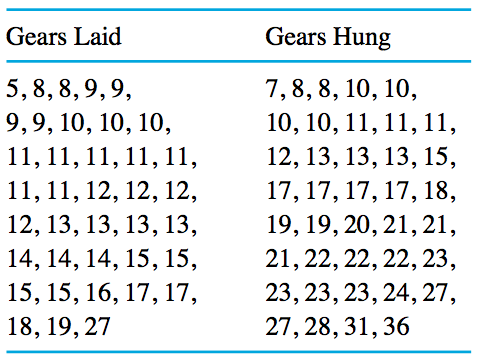
\includegraphics{../../fig/gearstable.png} 
\end{center}

\end{frame}

\begin{frame}
\frametitle{Summary}
\begin{center}
\setkeys{Gin}{width=.4\textwidth} 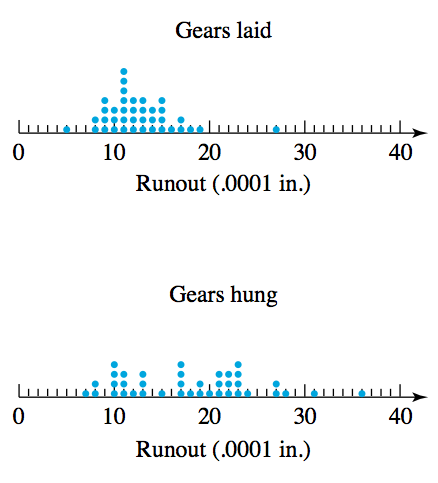
\includegraphics{../../fig/gearsdot.png} 
\end{center}

Mean laid runout: 12.6 $\times 10^{-4}$ in \q
Mean hung runout: 17.9  $\times 10^{-4}$ in
\end{frame}


\begin{frame}
\frametitle{Inference and Interpretation}
\begin{itemize}
\item Inference uses probability theory, symbols, and equations to answer questions like:
\begin{itemize}
\item Can we be confident that the ``true" mean laid runout is within $2.0 \times 10^{-4}$ of our observed mean of 12.6 $\times 10^{-4}$ in? \pause
\item Is the mean laid runout significantly lower than the mean hung runout? 
\end{itemize} \pause
\item Interpretation explains those answers in layman's terms without all the probability theory, symbols and equations.
\end{itemize}
\end{frame}

\section{Populations and Samples}

\begin{frame}
\frametitle{Populations and Samples}
\begin{itemize}
\item Definitions
\begin{itemize}
\item {\bf Sample}: the collection of objects (most relevant to the central goals of the study) selected for direct measurement.  
\pause \item {\bf Population}: the bigger group of things or people from which the sample was taken. 
\end{itemize}
\pause \item Gears study
\begin{itemize}
\item Sample: the 77 gears arranged, tested, and measured for distortion
\pause \item Population: All the gears with the same make and model as those included in the experiment.
\end{itemize}
\end{itemize}
\end{frame}

\begin{frame}
\frametitle{Your turn: state the sample and the population.} \small
\begin{itemize}
\item On Dec. 1-2, 2012, the \href{http://www.gallup.com/}{Gallup Poll} conducted a \href{http://www.gallup.com/poll/159065/americans-widely-prefer-compromise-fiscal-cliff.aspx}{study} to find out what proportion of Americans prefer a compromise on the Fiscal Cliff issue. 
\pause \item 1000 adults were randomly selected for telephone interviews. The adults were aged 18 and older and living in any of the 50 U.S. states or the District of Columbia.
\end{itemize}
\end{frame}

\begin{frame}<handout:\answers>
\frametitle{Answers}
\begin{itemize}
\item Sample: the 1000 adults selected.
\pause \item Population: All adults aged 18 and older who live in any of the 50 U.S. states or the District of Columbia.
\end{itemize}
\end{frame}


\begin{frame}
\frametitle{Your turn: state the sample and the population.} \small
\begin{itemize}
\item \href{http://www.esbit.net/}{Esbit} manufactures fuel pellets out of compressed hexamine powder. Suppose a new shipment of 100 pelletizing machines arrives, and the goal of a new study is to determine the quality of this particular new shipment. 
\pause \item 5 machines out of the 100 are randomly selected for comprehensive testing in which each produces 200 pellets, and each pellet's mass, volume, flash point, and rate of combustion are measured.
\end{itemize}
\end{frame}

\begin{frame}<handout:\answers>
\frametitle{Answers}
\begin{itemize}
\item Sample: The 5 pelletizing machines selected for testing.
\pause \item Population: The new shipment of 100 pelletizing machines.
\end{itemize}
\end{frame}







\section{Data and Measurement}

\begin{frame}
\frametitle{Measurement issues}

A measurement system is:
\begin{itemize}
\item {\bf Valid} if it usefully and appropriately represents the feature  of interest.
\pause \item {\bf Accurate} if it produces the correct value on average. 
\pause \item {\bf Precise} if there is little variation in repeated measurements of the same object. 
\end{itemize}
\end{frame}



\begin{frame}
\frametitle{Example: paper} \scriptsize
Two students measured the thickness of paper in the same book. Each student took 10 measurements.

\begin{center}
\setkeys{Gin}{width=.55\textwidth} 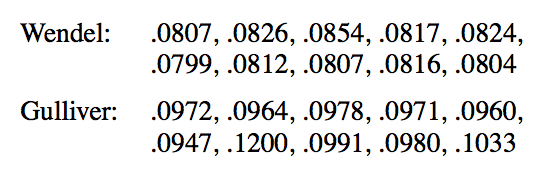
\includegraphics{../../fig/papertable.png} \q 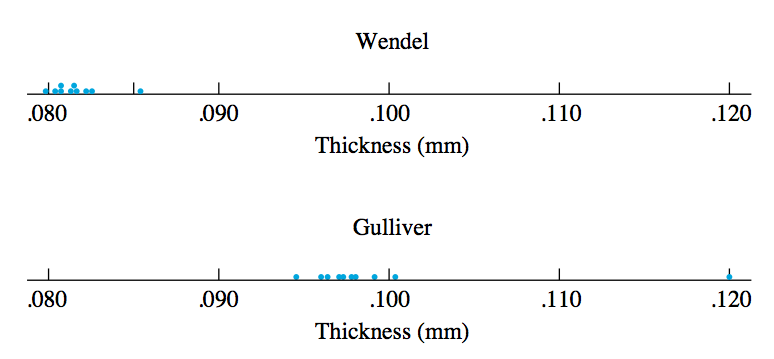
\includegraphics{../../fig/paperdot.png} 
\end{center}

\pause If the true thickness of the paper is 0.1 mm, then:

\begin{enumerate}
\item Who is more accurate?
\item Who is more precise?
\end{enumerate}
\end{frame}

\begin{frame}
\frametitle{Example: paper}

\begin{enumerate}[1. ]
\item Gulliver is more accurate because his measurements are closer to 0.1 mm on average.
\pause \item Wendel is more precise because her measurement s are less varied.
\end{enumerate}
\end{frame}

\begin{frame}
\frametitle{Types of data}
\vspace{-0.5em}
{\small
\begin{itemize}
\item {\bf Categorical (qualitative)}: Each measurement is a non-numerical value (male or female, operating condition A or B, green or blue).
\pause \item {\bf Numerical (quantitative)}: Each measurement is a number (thrust face runout of gears, mass of fuel pellets)
\begin{itemize}
\pause \item {\bf Discrete}: measurements are separated points (number of pages in a book, number of shark attacks, CPU FLOPs per day, credit card numbers)
\pause \item {\bf Continuous}: measurements lie on a continuum (mass of fuel pellets, mpg of a car, thrust face runout of gears)
\end{itemize}
\pause \item {\bf Univariate}: one measurement per sample unit
\pause \item {\bf Multivariate}: multiple measurements per sample unit (2 measurements = bivariate data)
\pause \item {\bf Paired Data}: bivariate data where both variables are attempting to quantify the "same thing" - often, before + after (e.g. like metal specimen hardness before and after heat treating) or measurements of the same quantity made with different instrucments/systems
\end{itemize}
}
\end{frame}


\begin{frame}
\frametitle{Gears runout data: univariate or bivariate?}

\begin{center}
\setkeys{Gin}{width=.75\textwidth} 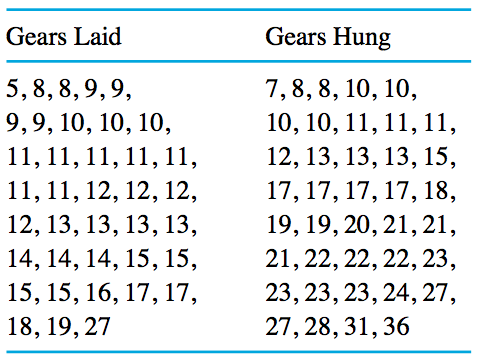
\includegraphics{../../fig/gearstable.png} 
\end{center}

\end{frame}

\begin{frame}[fragile]
\frametitle{Answer: bivariate}

 \small
Arrange the data in a table, where:
\begin{itemize}
\item Each row is a {\bf sample unit}, or thing that you measure (gear, in this case).
\pause \item Each column is a {\bf variable}, or characteristic that you control or measure.
\end{itemize}

\pause \begin{center}
\begin{tabular}{cc}
Arrangement & Runout \\ \hline
laid & 5 \\
laid & 8 \\ 
laid & 8 \\ 
laid & 9 \\
laid & 9 \\ 
$\vdots$ & $\vdots$ \\ 
hung & 31 \\ 
hung & 36 \\
\end{tabular}
\end{center} 

This ``sample unit $\times$ variable" arrangement is the standard way to display data, and it helps account for all the variables.

\end{frame}

\section{Variables}

\begin{frame}
\frametitle{Variables} \scriptsize

\begin{itemize}
\item  {\bf Variable}: a characteristic that you control or measure
\pause \item {\bf Level}: a possible value of a variable
\end{itemize}

\pause Types of variables:

\begin{itemize}
\item {\bf Treatment variable}: a variable that the experimenter sets by acting on the sample (gear arrangement: laid or hung).
\begin{itemize}
\pause \item This action on the sample is called a {\bf treatment} (laying or hanging the gears).
\pause \item Treatment levels divide the sample into {\bf treatment groups} (laid gears and hung gears).
\end{itemize}
\pause \item {\bf Concomitant variable}: a passively measured variable (i.e., runout)
\pause \item {\bf Factor}: any discrete or categorical variable with a finite set of possible levels (operating condition A, B, or C for a chemical process)
\pause \item {\bf Response variable}: the outcome or result of a study (i.e., runout)
\pause \item {\bf Predictor variable (predictor, covariate)}: any variable that is not the response
\end{itemize}
\end{frame}


\begin{frame}
\frametitle{Blocking variables}

{\bf Blocking variable}: a discrete concomitant variable that describes some innate characteristic of the sample before treatment (gear size: big or small).  
\begin{itemize}
\pause \item Blocking variables divide the sample into smaller samples called {\bf blocks} (big gears and small gears).
\pause \item In practice, each block is collected as a separate sample. (Take a sample of big gears from a population of big gears, and then take a sample of small gears from a population of small gears.)
\end{itemize}
\end{frame}

\section{Experimental vs. Observational Studies}

\begin{frame}
\begin{itemize}
\item {\bf Experimental study (experiment)}: a study with at least one treatment variable: i.e., one in which the investigator acts on the sample in some way.
\pause \item {\bf Observational study}: a study with no treatment variables: all variables are concomitant, and all phenomena are passively observed.
\end{itemize}
\end{frame}

\begin{frame}
\frametitle{Example: metallurgy} \scriptsize

\begin{itemize}
\item A senior design class in metallurgical engineering took on the project of helping a manufacturer determine the brittleness of a spike-shaped metal part. The manufacturer wants these parts to bend with impact rather than shatter. 
\pause \item Each spike was hit with a swinging arm, and the response (bend or shatter) was recorded. The angle past vertical of the swinging arm varied among spikes. 
\pause \item Some spikes were made of metal A, others were made of metal B.
\pause \item The experimental conditions $-$ i.e., the temperature of the room, the force holding the spikes in place, etc. $-$ were held constant across levels of the arm.
\end{itemize}

 

\begin{center}
\setkeys{Gin}{width=.4\textwidth} 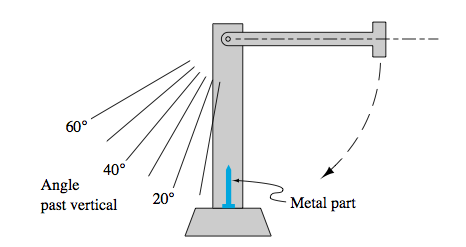
\includegraphics{../../fig/brittleschematic.png}
\end{center}

\pause Is this an experiment or an observational study? Identify and classify all the variables.

\end{frame}

\begin{frame}
\frametitle{Example: metallurgy}
\begin{itemize}
\item The study is an experiment. 
\pause \item Variables:
\begin{itemize}
\item Treatment variable: swinging arm angle.
\pause \item Blocking variable: material of the spike.
\pause \item Response variable: post-impact status of the spike: bent or shattered.
\end{itemize}

\pause \item Suppose we find:
\begin{itemize}
\item The higher the swinging arm, the more often the spikes shattered.
\pause \item Fewer metal A spikes shattered than metal B spikes.
\end{itemize}
\pause \item Answer the following:
\begin{enumerate}
\item Does raising the swinging arm higher CAUSE more parts to be shattered?
\pause \item Is metal A better than metal B for making minimally brittle spikes?
\end{enumerate}
\end{itemize}
\end{frame}

\begin{frame}
\frametitle{Example: metallurgy}
\begin{enumerate}[1. ]
\item Yes: the experimenter controlled the swinging arm, and the level of the arm was not correlated with any experimental conditions.
\item Not in this case: 
\begin{itemize}
\item Metal A (titanium) is more brittle than metal B (steel).
\item The titanium spikes were made from a good manufacturer, and the steel spikes were made from a terrible manufacturer. 
\end{itemize}
\end{enumerate}

Notice: 
\begin{itemize}
\item Metal type is not a treatment variable.
\item Metal type was correlated with a {\bf lurking variable}: the identity of the manufacturer.
\end{itemize}
\end{frame}


\begin{frame}
\frametitle{Causality in studies}

You can only infer causality when:
\begin{enumerate}[1. ]
\item The prospective cause is a treatment variable.
\pause \item If all possible predictors are uncorrelated with the treatment variable. \pause (i.e., if you can't predict the treatment variable based on experimental conditions.)
\end{enumerate}

\pause That means:

\begin{itemize}
\item You cannot infer causality in an observational study.
\pause \item In an experiment, you can infer causality between the response and a treatment if:
\begin{itemize}
\pause \item All the experimental conditions are controlled, or:
\pause \item The investigator randomly assigns sample units to treatment levels in a way that does not depend on experimental conditions. 
\end{itemize}
\end{itemize}
\end{frame}

\begin{frame}
\frametitle{Example: sales data}

An analyst at Kmart looked at the last five years of sales data. He discovered that sales were high on days when the displays were mostly red and low on days when the displays were mostly blue. 

\begin{enumerate}
\pause \item Is this an experimental or observational study?
\pause \item Does replacing blue with red in the displays cause sales to improve?
\end{enumerate}

\end{frame}

\begin{frame}
\frametitle{Example: sales data}

\begin{enumerate}[1. ]
\item This is an observational study.
\pause \item No. Displays were red around Christmas time and blue otherwise. The spike in sales was caused by the holiday season, not the display color. 
\end{enumerate}

\pause The display color:
\begin{itemize}
\item Was not a treatment variable.
\pause \item Was correlated with the schedule of holidays.
\end{itemize}
\end{frame}

\begin{frame}
\frametitle{Example: rat data}
\small
A biologist studied the effect of a growth hormone on weight gain in rats. 600 rats were selected for the study. The rats varied greatly in:
\begin{itemize}
\pause \item Age (Younger ones gain weight faster)
\pause \item Breed (Breed A grows faster than breed B.)
\pause \item origin (Either biology lab or the wilderness. Let's say lab rats grow faster.)
\end{itemize}
\pause However, none of these factors were taken into account in the study. Instead, 300 rats were randomly selected from the original 600 to receive the hormone. The others received a placebo. \pause At the end of three months, the rats with the hormone gained more weight than the rats without the hormone on average.

\begin{enumerate}[1. ]
\pause \item Is this an experiment or an observational study?
\pause \item Does the hormone cause weight gain in rats?
\end{enumerate}
\end{frame}


\begin{frame}
\frametitle{Answers}
\begin{enumerate}[1. ]
\pause \item Experimental study.
\pause \item The hormone \emph{does} cause weight gain in rats.
\begin{itemize}
\pause \item The hormone was a treatment.
\pause \item Age, breed, and origin, and all other experimental conditions are \emph{constant on average} with hormone level. That's because we randomly selected rats to receive the hormone
\pause \item In addition, since the treatment groups are large, the conditions are \emph{approximately constant} with hormone level.
\end{itemize}
\end{enumerate}
\end{frame}

%\begin{frame}
%\frametitle{Sources}
%\begin{enumerate}[1. ]
%\item Some source
%\end{enumerate}
%\end{frame}

\end{document}
